\documentclass[border=2pt]{standalone}
\usepackage{tikz}

\begin{document}

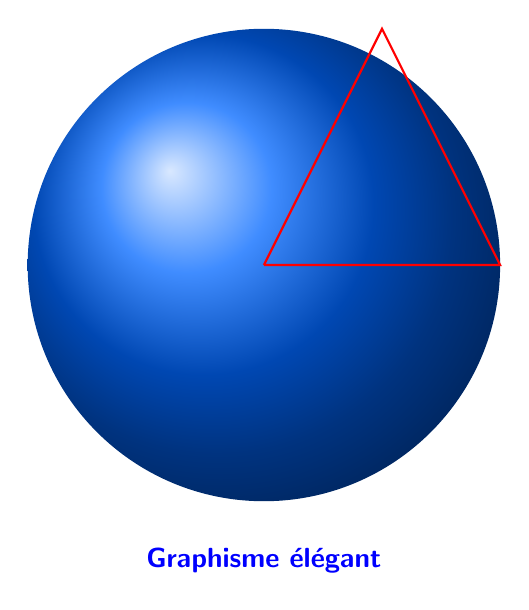
\begin{tikzpicture}[scale=1.5]
    % Dessin d'un cercle avec un dégradé de couleur
    \shade[ball color=cyan!40!blue] (0,0) circle (2);
    
    % Dessiner une étoile avec des traits épais
    \draw[thick, red] (0,0) -- (1,2) -- (2,0) -- (0,0);
    
    % Texte stylisé sur la figure
    \node[align=center, font=\sffamily\bfseries, blue] at (0,-2.5) {Graphisme élégant};
\end{tikzpicture}

\end{document}
